\chapter{Παρατηρησιακά χαρακτηριστικά αστέρων}
\label{ch:Chapter2}

\section{Μέθοδος της παράλλαξης}
% Πόσο μακριά είναι τα αστέρια; %
% ----------------------------- %

\textbf{Πως μετράμε αποστάσεις μέσα στο ηλιακό σύστημα;}\\
Με τη βοήθεια των radar. Στέλνουμε μία δέσμη φωτονίων στα ραδιαφωνικά μήκη κύματος, τα φωτόνια αυτά ανακλώνται από την επιφάνεια του πλανήτη ή του Ήλιου, επιστρέφουν σε εμάς και εφόσον γνωρίζουμε το χρονικό διάστημα που παρήλθε από τη στιγμή της εκπομπής του σήματος εώς τη λήψη του, η απόσταση θα δίνεται απλά:

\begin{equation}
    d = c (\delta t / 2)
\end{equation}
όπου $c$ είναι η ταχύτητα του φωτός και $\delta t$ το χρονικό διάστημα ανάμεσα στην εκπομπή και τη λήψη του σήματος.
\\
%{\color{red} \rule{\linewidth}{0.2mm} }
{\color{red} \hrule}
Αυτός ο τρόπος μέτρησης αποστάσεων ισχύει μόνο για αντικείμενα μέσα στο ηλιακό μας σύστημα και δεν μπορεί να χρησιμοποιηθεί για τον υπολογισμό αποστάσεων άλλων αστέρων. Λόγω των τεράστιων αποστάσεων, το σήμα θα έπρεπε να ταξιδεύει για χρόνια μέχρι να φτάσει (x2 μέχρι να γυρίσει) στον αστέρα.
Επίσης, το σήμα θα ήταν πολύ εξασθενημένο για να μετρηθεί πίσω στη Γη.
{\color{red} \hrule }


Μέσω αυτής της μεθόδου, ξέρουμε ότι η \textit{μέση} απόσταση Γης-Ήλιου είναι: $$1 \ \text{AU} \approx 149600000 \ \text{km}$$

Για να μετράμε αποστάσεις σχετικά κοντινών αστέρων, χρησιμοποιούμε την μέθοδο της \textit{παράλλαξης}. Η μέθοδος αυτή βασίζεται στην \textit{φαινόμενη} κίνηση ενός αντικειμένου σε σχέση με ένα πολύ πιο μακρινό υπόβαθρο (background) καθώς το κοιτάμε από διαφορετικές γωνίες. Με άλλα λόγια, η παράλλαξη είναι η φαινόμενη αλλαγή στη θέση ενός αντικειμένου βάσει μιας διαφορετικής οπτικής γωνίας.

\textit{\underline{Παράδειγμα}}: Κρατήστε το δάχτυλό σας μπροστά από το πρόσωπό σας και παρατηρείστε το ανοιγοκλείνωντας ένα μάτι κάθε φορά. Όσο μεγαλύτερη είναι η απόσταση στην οποία τοποθετούμε το δάχτυλο, τόσο μικρότερη είναι η φαινόμενη μετατόπιση λόγω της διαφορετικής θέσης της παρατήρησης.
\hrule

Χρησιμοποιώντας την παραπάνω γεωμετρική ιδιότητα, παρατηρούμε ότι κοντινά αστέρια φαίνεται να μετατοπίζονται λόγω της κίνησης της Γης γύρω από τον Ήλιο (σχήμα \ref{fig:parallax}).

\begin{figure}[h]
    \centering
    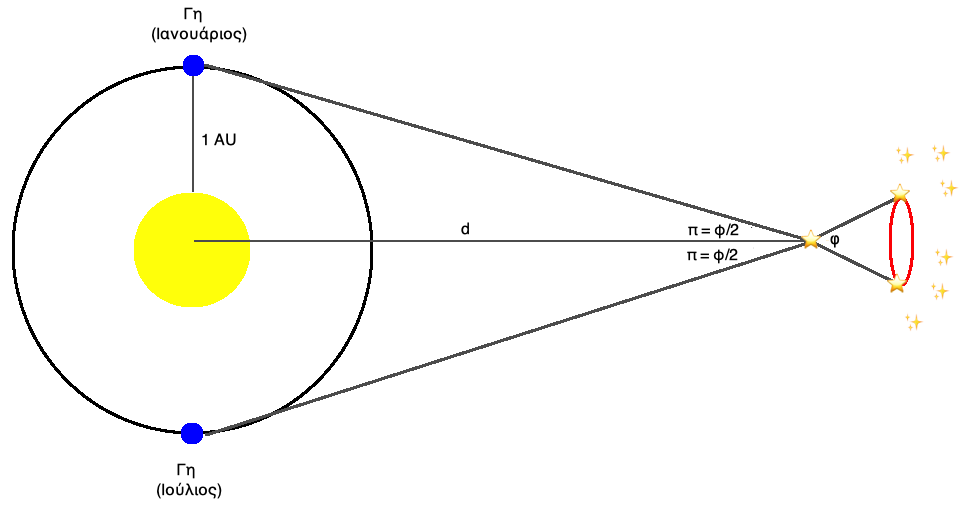
\includegraphics[width=\linewidth]{Figures/parallax.png}
    \caption{Ορισμός της ετήσιας παράλλαξης.}
    \label{fig:parallax}
\end{figure}

Μετράμε την θέση ενός στόχου-αστέρα και την ξαναμετράμε έπειτα από 6 μήνες όταν η Γη θα βρίσκεται στην αντιδιαμετρική θέση της τροχιάς της. Στη συνέχεια, μετράμε την αλλαγή στη φαινόμενη θέση του αστέρα σε σχέση με κάποια πολύ μακρινά άστρα στο υπόβαθρο που η φαινόμενη μετατόπισή τους είναι αμελητέα. Αυτή η αλλαγή περιγράφεται σε όρους "γωνία παράλλαξης", $\pi$. Για μία φαινόμενη μετατόπιση $\phi$, η απόσταση $d$ του στόχου δίνεται από:

\begin{equation}
    d = \frac{1 \ \text{AU}}{\tan \pi} \approx \frac{1 \ \text{AU}}{\pi}
\end{equation}
όπου στο δεύτερο μέρος χρησιμοποιήσαμε τη σχέση για μικρές γωνίες (small angle approximation) $\tan \theta \approx \theta$, όταν η γωνία $\theta$ μετριέται σε \textit{ακτίνια} (rad).

Η κόκκινη έλλειψη στο σχήμα υποδηλώνει την φαινόμενη ελλειπτική τροχιά που εκτελεί ο αστέρας πάνω στην ουράνια σφαίρα, λόγω της περιστροφής της Γης γύρω από τον Ήλιο. Αυτο το γεγονός είναι και μια άμεση απόδειξη ότι η Γη κινείται γύρω από τον Ήλιο και όχι το ανάποδο.
\\
{\color{red} \hrule }
Το γεγονός ότι η τροχιά της Γης δεν ειναι απόλυτα σφαιρική δεν αποτελεί ιδιαίτερο πρόβλημα καθώς οι διακυμάνσεις στην ακτίνα της τροχιάς είναι πάρα πολύ μικρές συγκριτικά με την απόσταση $d$ των αστέρων. Άλλωστε, το σφάλμα στην μέτρηση της παράλλαξης είναι πολύ μεγαλύτερο από το σφάλμα που υπεισέρχεται εαν θεωρήσουμε ότι η ακτίνα της τροχιάς της Γης γύρω από τον Ήλιο δεν παραμένει σταθερή.
{\color{red} \hrule }

Γνωρίζουμε ότι $1 \ \text{rad} = 57.3^{\circ} = 206265 \ \text{arcsec}$. Μπορούμε να ορίσουμε έτσι, ένα νέο μέγεθος για μέτρηση μήκους, το \textit{parsec} (pc). Ένα parsec ορίζεται ως η απόσταση ενός αντικειμένου το οποίο πρέπει να έχει ώστε να παράγει παράλλαξη (parallax shift) ίση με 1 arcsec.

\begin{equation}
    1 \ \text{pc} = \frac{1 \ \text{AU}}{4.85 \times 10^{-6} \ \text{rad}} = 3.09 \times 10^{18} \ \text{cm} = 3.26 \ \text{ly}
\end{equation}

Έτσι, ισχύου οι σχέσεις:

\begin{equation}
    d = \frac{1 \ \text{AU}}{\pi \ (\text{rad})} = \frac{206265 \ \text{AU}}{\pi \ (\text{arcsec})} = \frac{1 \ \text{pc}}{\pi \ (\text{arcsec})}
\end{equation}
\textit{\underline{ΠΡΟΣΟΧΗ}}: Η ΓΩΝΙΑ $\pi$ ΑΝΑΦΕΡΕΤΑΙ ΣΤΗΝ ΠΑΡΑΛΑΞΗ ΚΑΙ ΟΧΙ ΣΤΗΝ ΣΤΑΘΕΡΑ!
\\
{\color{red} \hrule }
E: Γιατί να ορίσουμε το parsec με βάση παράλλαξη $\pi = 1 \ \text{arcsec}$;\\
Α: Γιατί το κοντινότερο σε μας αστέρι (Εγγύτατος του Κενταύρου) έχει παράλλαξη $\pi \simeq 1 \ \text{arcsec}$, άρα όλα τα άλλα αστέρια είναι πολλαπλάσια του 1pc.
{\color{red} \hrule }

\textit{\underline{Παράδειγμα}}: Ο εγγύτατος του Κενταύρου έχει παράλλαξη $ \pi = 0.77 \ \text{arcsec}$. Άρα η απόστασή του είναι:
\begin{equation*}
    d = \frac{1}{\pi \ \text{arcsec}} \text{pc} = \frac{1}{0.77} \ \text{pc} = 1.3 \ \text{pc} \simeq 267000 \ \text{AU}
\end{equation*}
\hrule



\section{Λαμπρότητα αστέρων}
% Πόσο λαμπρά είναι τα αστέρια; %
% ----------------------------- %

Η συντριπτική πλειοψηφία των πληροφοριών που έχουμε για τα αστέρια είναι μέσω της συλλογής φωτός σε διάφορα μήκη κύματος. Η έλλειψη φωτεινής πληροφορίας (ενώ ξέρουμε ότι έχει εκπεμφθεί) μας τροφοδοτεί με περαιτέρω πληροφορία για τις διαδικασίες απορρόφησης αυτής της μερίδας Η/Μ κυμάτων από τη μεσοαστρική ύλη.

Όταν μετράμε το φως που εκπέμπουν τα άστρα, μετράμε:
\begin{enumerate}
    \item την ένταση
    \item την πόλωση
\end{enumerate}

Η προφανής και πρώτη ερώτηση που μας έρχεται στο μυαλό είναι:
``Όλα τα αστέρια έχουν την ίδια λαμπρότητα, και γιατί;''. Ξερουμε ότι ενδογενώς, όλα τα αστέρια δεν έχουν την ίδια λαμπρότητα. Αλλά και την ίδια λαμπρότητα να είχαν, αυτό σημαίνει ότι θα φαινόντουσαν το ίδιο λαμπρά σε εμάς; Τι ρόλο παίζει η απόσταση σε αυτή την εικόνα; Είναι προφανές ότι πρέπει να ορίσουμε κάποιες ποσότητες που έχουν να κάνουν τόσο με την ενδογενή, όσο και με την φαινόμενη λαμπρότητα του αστέρα.

Ως \textit{λαμπρότητα} (L) ορίζουμε τη συνολική ισχύς (ενέργεια/χρόνο) που ακτινοβολείται από την επιφάνεια του αστέρα. Ως ισχύς, η λαμπρότητα μετριέται σε [W, erg/s]. Με άλλα λόγια, η λαμπρότητα εκφράζει τον ρυθμό με τον οποίο ένα αστέρι ακτινοβολεί ενέργεια. Η λαμπρότητα είναι μια ενδογενής ιδιότητα και μπορεί να υπολογισθεί από την \textit{φωτεινότητα} (ροή ή φαινόμενη λαμπρότητα), την ενέργεια δηλαδή της Η/Μ ακτινοβολίας που φτάνει στη Γη, και μπορεί να μετρηθεί άμεσα. Η φωτεινότητα εξαρτάται από την απόσταση του αστέρα από εμάς και ορίζεται από τη σχέση:

\begin{equation}
    F = \frac{L}{4 \pi d^2}
\end{equation}
όπου $d$ η απόσταση του αστέρα από τη Γη.

Η ποσότητα $4 \pi d^2$ ορίζει ουσιαστικά μία επιφάνεια σφαίρας με ακτίνα $d$ (σχήμα \ref{fig:flux}), και άρα η φωτεινότητα είναι μια ποσότητα που μετριέται σε [W/$\text{m}^2$, $\text{erg} \cdot \text{s}^{-1} \cdot \text{cm}^{-2}$]. Μπορούμε να πούμε δηλαδή ότι η φωτεινότητα ενός αστέρα είναι η ενέργεια ανα μονάδα χρόνου που διέρχεται από επιφάνεια $1 \ \text{m}^2$, \textit{ανεξάρτητα} της διεύθυνσης διάδοσης του φωτός.

\begin{figure}[h]
    \centering
    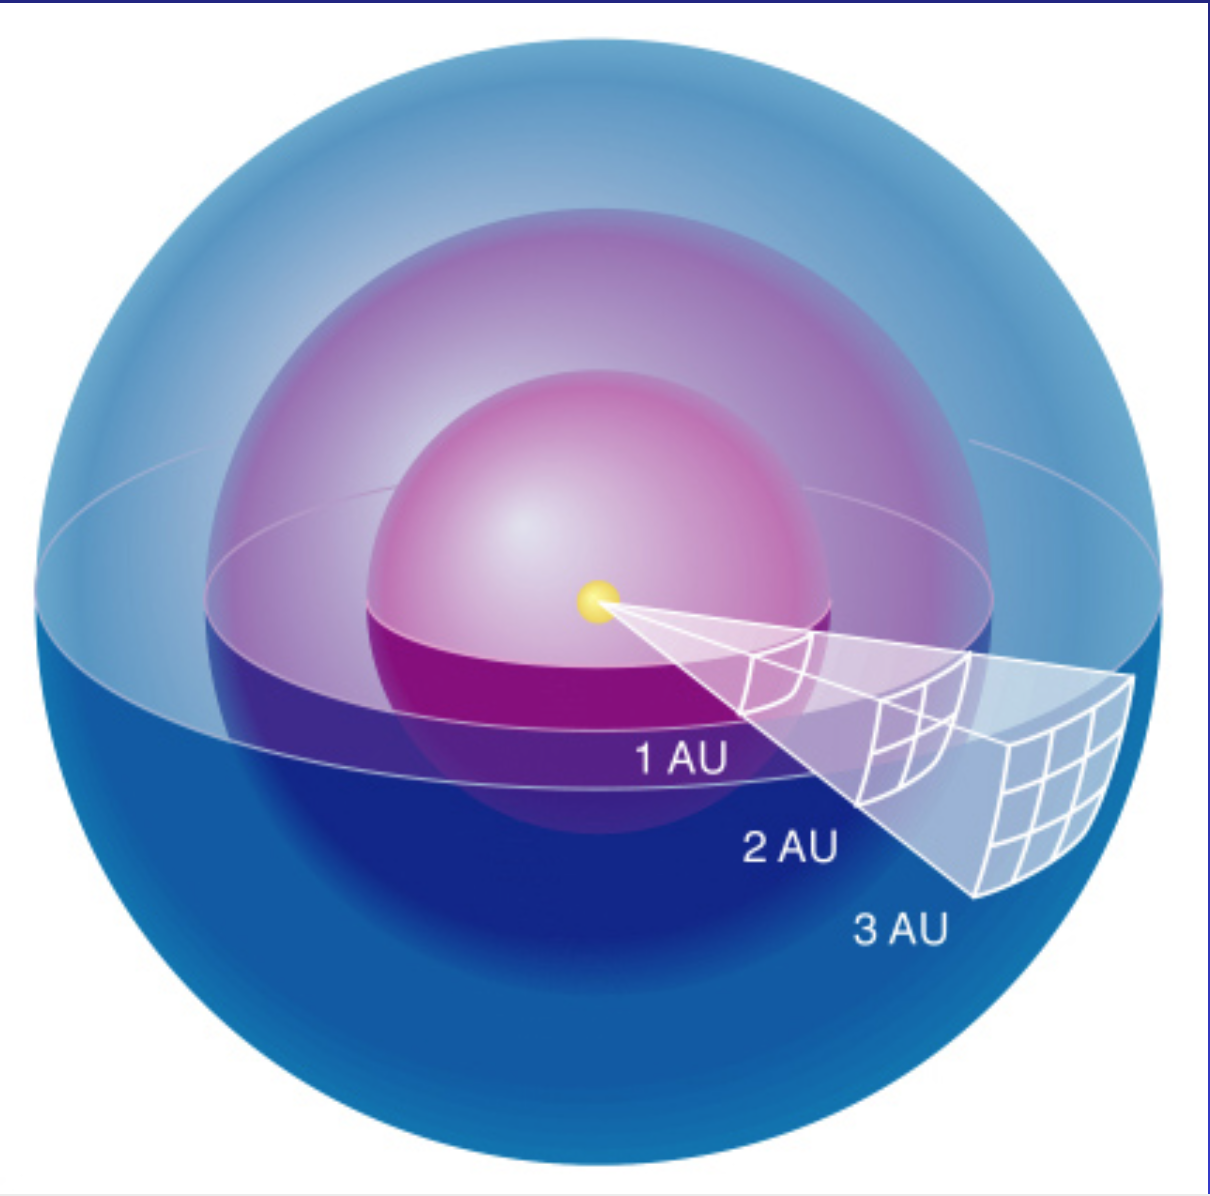
\includegraphics[scale=0.3]{Figures/flux.png}
    \caption{Φαινόμενη λαμπρότητα αστέρα και εξάρτησή της από την απόσταση.}
    \label{fig:flux}
\end{figure}

'Ενας τρόπος να ταξινομήσουμε τα αστέρια είναι ανάλογα με τη φωτεινότητά τους, δηλαδή με το πόσο λαμπρά φαίνονται στο ανθρώπινο μάτι (Ίππαρχος). Αργότερα, υιοθετήθηκε ένας μαθηματικός τύπος (Pogson) που μας δίνει το \textit{φαινόμενο μέγεθος} ενός αστέρα, δηλαδή του πόσο φωτεινός φαίνεται να είναι:

\begin{equation}
    \label{eq:apparent_magnitude}
    m = -2.5 \log \left ( \frac{F}{F_0} \right )
\end{equation}
όπου $F_0$ είναι μία σταθερά.

Παρατηρούμε ότι το μέγεθος ενός αστέρα δεν είναι τίποτα άλλο παρά η φωτεινότητά του εκφρασμένη σε λογαριθμική κλίμακα. Αυτό μας δίνει ένα μέτρο για τη μείωση της ροής της ακτινοβολίας λόγω της απόστασης, σύμφωνα με τον νόμο του αντίστροφου τετραγώνου.

Γιατί όμως το μέγεθος ως ποσότητα υπερτερεί έναντι της χρήσης της φωτεινότητας ως μέγεθος; Γιατί η φωτεινότητα ενός αστέρα που καταγράφει ένα τηλεσκόπιο εξαρτάται από το μέγεθος του κατόπτρου (ένα τηλεσκόπιο 10 μέτρων έχει δέκα φορές μεγαλύτερη συλλεκτική επιφάνεια από ένα τηλεσκόπιο 1 μέτρου), αλλά και από την ευαισθησία του εξοπλισμού (π.χ. μία μοντέρνα κάμερα μπορεί να καταγράφει περισσότερα φωτόνια ίδιας ενέργειας). {\color{blue} Προκύπτει άρα η ανάγκη βαθμονόμησης}. Η βαθμονόμηση αυτή γίνεται βάσει της φωτεινότητας του Vega ($F_0$) η οποία έχει γίνει σε πραγματικές μονάδες (W/$\text{m}^2$). Άρα χρησιμοποιώντας τον λόγο ($F/F_0$) προκύπτει ένα μέγεθος που δεν εξαρτάται από τον παρατηρησιακό εξοπλισμό.

Παραμένουν όμως οι ερωτήσεις: γιατί λογάριθμος, γιατί το μείον στη σχέση \eqref{eq:apparent_magnitude}, και γιατί ο συντελεστής 2.5; Γιατί να μην ορίζαμε το μέγεθος ως $m = F/F_0$ για παράδειγμα;

Λύνοντας την εξίσωση \eqref{eq:apparent_magnitude} για δύο αστέρες έχουμε:

\begin{eqnarray*}
    m_1 &=& -2.5 \log \left( \frac{F_1}{F_0} \right) \Rightarrow F_1 = F_0 \cdot 10^{-m_1/2.5} = F_0 \cdot 100^{-m_1/5} \\\\
    m_2 &=& -2.5 \log \left( \frac{F_2}{F_0} \right) \Rightarrow F_2 = F_0 \cdot 10^{-m_2/2.5} = F_0 \cdot 100^{-m_2/5}
\end{eqnarray*}
και διαιρώντας κατά μέλη παίρνουμε:

\begin{equation}
    \frac{F_1}{F_2} = 100^{(m_2 - m_1)/5}
\end{equation}

Παρατηρούμε ότι:
\begin{enumerate}
    \item αν οι δύο αστέρες διαφέρουν σε μέγεθος κατα 5, τότε η φωτεινότητά τους διαφέρει κατά έναν παράγοντα 100. Ο μαθηματικός που έκανε αυτή την παρατήρηση (Pogson), ήθελε να συνεχίσει την κλίμακα του Ίππαρχου όπου ένα αστέρι με μέγεθος 1 είναι 100 φορές πιο φωτεινό από ένα αστέρι με μέγεθος 6 ($\Delta m = 5$). Ο τρόπος για να το πετύχει αυτό ήταν να βάλει έναν παράγοντα 2.5 στη σχέση που συνδέει μέγεθος με φωτεινότητα, η οποία πρέπει να είναι λογαριθμική καθώς η ευαισθησία του ανθρώπινου ματιού στη φωτεινότητα μια πηγής είναι λογαριθμική.
    \item Αν $F_1 < F_2$ τοτε $m_1 > m_2$. Και πάλι, για να μην χαλάσει η ταξινόμηση του Ίππαρχου όπου τα πιο φωτεινά αστέρια είναι μικρότερου μεγέθους, προκύπτει το μείον στη σχέση \eqref{eq:apparent_magnitude}.
\end{enumerate}

Κατά αντιστοιχία, μπορούμε να ορίσουμε το \textit{απόλυτο μέγεθος}, M, ενός αστέρα ως το φαινόμενο μέγεθος (m) αν το αστέρι βρισκόταν σε απόσταση 10pc από εμάς.

\begin{eqnarray*}
    M &=& -2.5 \log \left( \frac{F_{10 \text{pc}}}{F_0} \right) \longrightarrow \frac{F_{10 \text{pc}}}{F} = 100^{(m-M)/5} \Rightarrow \\
    &\Rightarrow & \frac{\displaystyle L/4\pi (10 \text{pc})^2}{L/4 \pi d^2} = 100^{(m-M)/5} \Rightarrow d^2 = 100^{(m-M+5)/5} \Rightarrow \\\\
    & \Rightarrow & \boxed{d = 10^{(m-M+5)/5} \ \text{pc}}
\end{eqnarray*}
Λύνοντας ως προς $m-M$:

\begin{equation}
    \label{eq:distance_modulus}
    m-M = 5(\log d - 1)
\end{equation}

Η εξίσωση \eqref{eq:distance_modulus} είναι γνωστή ως \textit{distance modulus} και βάσει αυτής μπορούμε να υπολογίσουμε την απόσταση ενός αστέρα αν γνωρίζουμε το φαινόμενο και το πραγματικό μέγεθός του.

Στην περίπτωση που υπάρχει μεσοαστρική απορρόφηση, τότε η \eqref{eq:distance_modulus} γράφεται
\begin{equation}
    m - M - A = 5\log\,d - 5
\end{equation}
όπου $A$ είναι το μέγεθος της μεσοαστρικής απόσβεσης.

\section{Γωνιώδης απόσταση}
% Πόσο μεγάλα (σε όγκο) είναι τα αστέρια; %
% --------------------------------------- %
Υπάρχει ένας καθαρά γεωμετρικός τρόπος να υπολογίσει κανείς την ακτίνα ενός άστρου. Η μέθοδος αυτή βασίζεται στην \textit{γωνιακή διάμετρο} του αστέρα.

\begin{figure}[h]
    \centering
    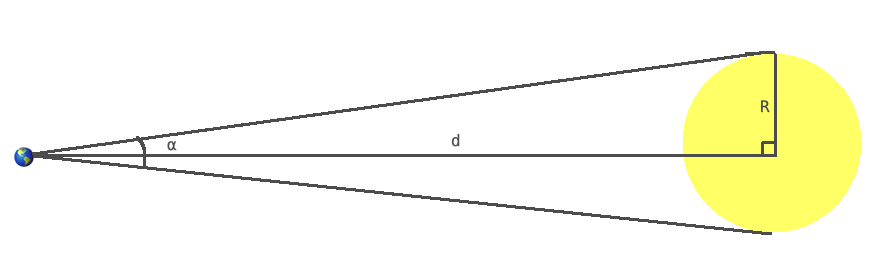
\includegraphics[scale=0.4]{Figures/angular_diameter.png}
    \caption{Γωνιακή διάμετρος α, ενός αστέρα. }
    \label{fig:angular_diameter}
\end{figure}

Από τη γεωμετρία του σχήματος \ref{fig:angular_diameter} παρατηρούμε ότι η γωνιακή διάμετρος α (κατά αναλογία, α/2 είναι η γωνιακή ακτίνα) θα δίνεται από τη σχέση:

\begin{equation}
    \label{eq:angular_diameter}
    \tan \left( \frac{\alpha}{2} \right) = \frac{R}{d}
\end{equation}
ενώ για μικρές γωνίες ισχύει: $\tan \theta \approx \sin \theta \approx \theta$, οταν η γωνία μετριέται σε ακτίνια.
\\

{\color{red} \hrule}
\textbf{Για τον Ήλιο}: $\alpha = 1919 \ \text{arcsec} = 31.98 \ \text{arcmin} = 0.53^{\circ} = 9.3 \times 10^{-3} \ \text{rad}$.

Άρα: $R_\odot = 1 \ \text{AU} \times \tan \left( \frac{0.53^{\circ}}{2}\right) \approx 0.0046 \ \text{AU}$

\textbf{Για τον Betelgeuse}: $\alpha = 0.125 \ \text{arcsec} = 0.0021 \ \text{arcmin} = 0.000035^{\circ}$, \\ $d=197 \ \text{pc} \simeq 4 \times 10^7 \ \text{AU} \ (\pm 45 \ \text{pc})$

Άρα: $R_B = (4 \times 10^7 \ \text{AU}) \times \tan \left( \frac{0.000035}{2} \right) \simeq 12 \ \text{AU} \Rightarrow R_B \simeq 2580 R_\odot$

O Betelgeuse είναι ένας υπεργίγαντας αστέρας με ακτίνα (και λαμπρότητα) κατά πολύ μεγαλύτερη από αυτή του Ήλιου.

\textbf{Για τον εγγύτατο του Κενταύρου}: $\alpha = 1 \times 10^{-3} \ \text{arcsec}$, $d = 1.3 \ \text{pc}$

Άρα: $R_{PC} \simeq 0.14 R_{\odot}$

Ο εγγύτατος του Κενταύρου είναι ένας νάνος αστέρας με ακτίνα (και λαμπρότητα) κατά πολύ μικρότερη από αυτή του Ήλιου.
{\color{red} \hrule}

Γίνεται αντιληπτό ότι ο άμεσος προσδιορισμός της γωνιακής διαμέτρου των αστέρων είναι εξαιρετικά δύσκολη υπόθεση λόγω της τεράστιας απόστασής τους.


\section{Σχέσεις $\rm L = f(M)$ και $\rm R = f(M)$}
Η πιο σημαντική θεμελιώδης ιδιότητητα, η μάζα, δεν μπορεί να μετρηθεί άμεσα για ένα απομονωμένο αστέρι. Για να μετρήσουμε αστρικές μάζες χρειαζόμαστε διπλά συστήματα αστέρων που παρουσιάζουν διακυμάνσεις στην ακτινική τους ταχύτητα (φασματοσκοπικά διπλοί αστέρες). Οι ακτινικές ταχύτητες από μόνες τους μπορούν να προσδιορίσουν μάζες μέχρι έναν παράγοντα $\sin i$, όπου $i$ είναι η γωνία κλίσης (inclination) της τροχιάς του διπλού συστήματος. Για τον προσδιορισμό απόλυτων τιμών της μάζας χρειαζόμαστε πληροφορίες για το $i$, είτε από ένα οπτικά διπλό σύστημα (visual binary) ή από την παρουσία εκλείψεων (eclipsing binary). Περισσότερα γι' αυτά τα συστήματα στο Κεφάλαιο  \ref{ch:Chapter7}. 

Από παρατηρήσεις άστρων στη γειτονιά του Ήλιου έχουμε καταφέρει να μετρήσουμε με ακρίβεια τις μάζες, τις λαμπρότητες και τις ακτίνες τους (σε διπλά συστήματα). Θα περίμενε κανείς να μην υπάρχει κανένας συσχετισμός μεταξύ αυτών των ποσοτήτων (λαμπρότητα και ακτίνα σχετίζονται μέσω του νόμου Stefan-Boltzmann οπως θα δούμε παρακάτω). Παρόλα αυτά, όταν κάνουμε τη γραφική παράσταση της λαμπρότητας με τη μάζα, και της ακτίνας με τη μάζα παρατηρούμε ότι υπάρχει ξεκάθαρα συχετισμός μεταξύ αυτών των ποσοτήτων (σχήμα \ref{fig:luminosity_mass_relation}).

\begin{figure}[h]
    \centering
    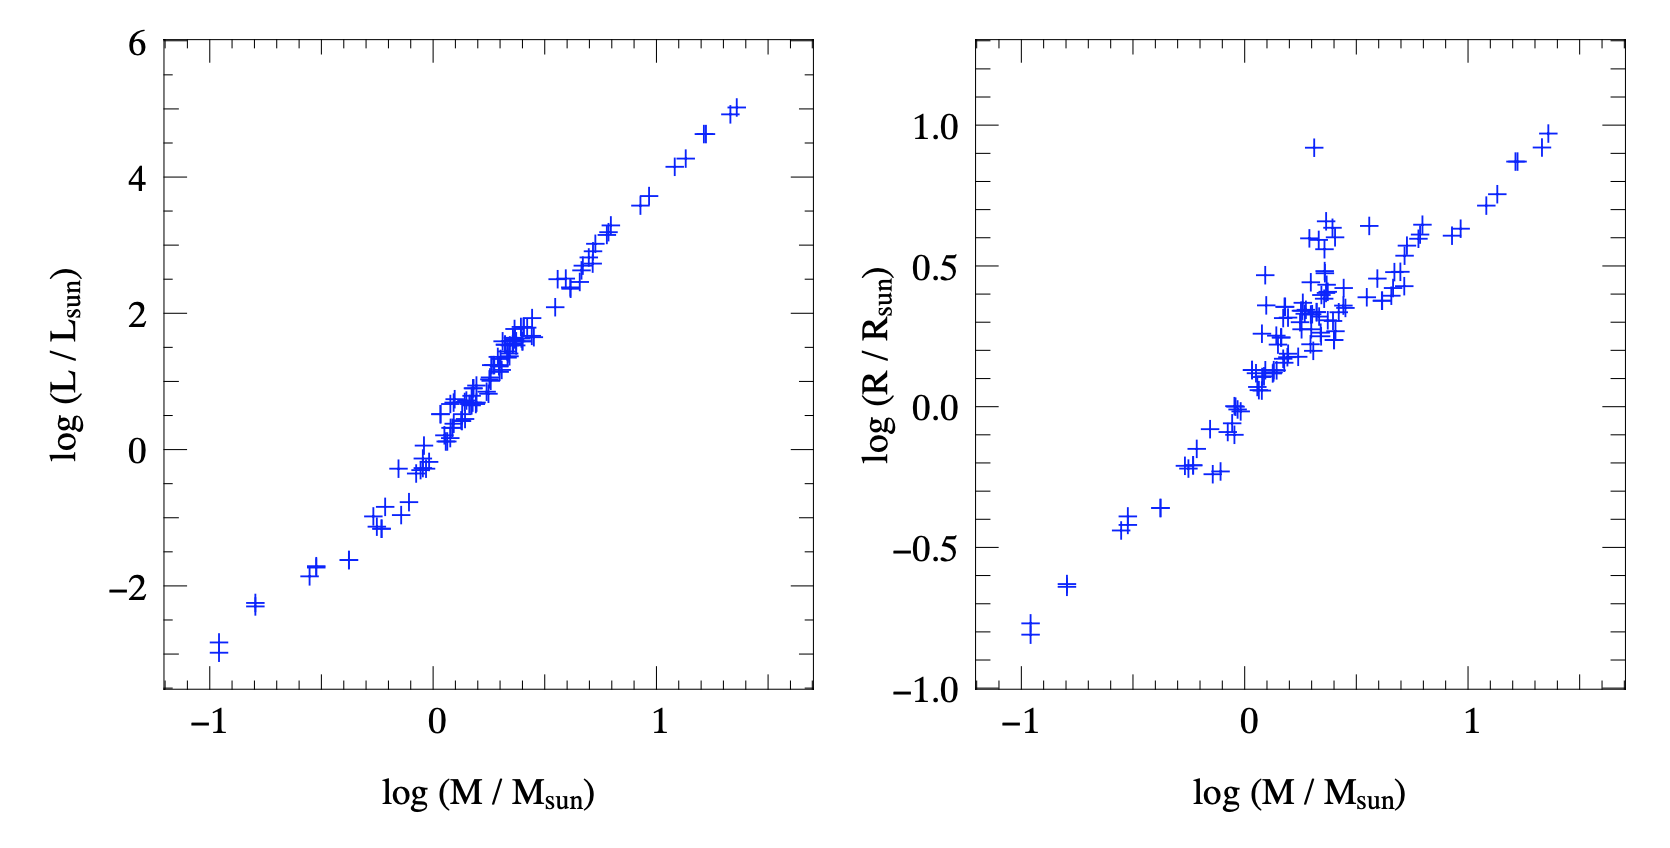
\includegraphics[width=\linewidth]{Figures/luminosity_mass_relation.png}
    \caption{Οι μάζες, ακτίνες και λαμπρότητες έχουν μετρηθεί με ακρίβεια $\lesssim 2 \,\%$ σε εκλειπτικά διπλούς αστέρες. Τα περισσότερα από αυτά τα αστέρια είναι αστέρες στην κύρια ακολουθία. Η διασπορά στις ακτίνες των αστέρων μεταξύ 1 και 2 $M_{\odot}$ οφείλεται στο γεγονός ότι αρκετά εξελιγμένα άστρα σε αυτό το εύρος μαζών, ικανοποιούν επίσης το κριτήριο της ακρίβειας της τάξης του $2 \,\%$.}
    \label{fig:luminosity_mass_relation}
\end{figure}

Αυτός ο παρατηρούμενος συσχετισμός μπορεί να προσεγγιστεί ικανοποιητικά καλά από τους εκθετικούς νόμους (power laws) των σχέσεων \eqref{eq:lum_mass} και \eqref{eq:radius_mass}.

\begin{equation}
    \label{eq:lum_mass}
    L \propto 
    \begin{cases}
        M^{2.5} & \text{εαν} \ M < 0.7 M_{\odot} \\\\
        M^{3.8} & \text{εαν} \ M > M_{\odot}
    \end{cases}
\end{equation}

\begin{equation}
    \label{eq:radius_mass}
    R \propto M^{0.7}
\end{equation}

Προφανώς, χρειαζόμαστε μία θεωρία αστρικής εξέλιξης η οποία να εξηγεί την ύπαρξη και τις κλίσεις αυτών των σχέσεων.


\section{Ακτινοβολία μέλανος σώματος}
% Πόσο ζεστά είναι τα αστέρια; %
% ---------------------------- %

{\color{red} \hrule}
Ε: Γιατί διάφορα αστέρια φαίνονται διαφορετικό χρώμα στον ουρανό; (π.χ. Rigel vs Betelegeuse)\\
A: Επειδή έχουν διαφορετικές θερμοκρασίες. Αυτός ο συσχετισμός δεν είναι προφανής, αλλά όπως θα δείξουμε στη συνέχεια, η συχνότητα εκπομπής ενός αντικειμένου εξαρτάται \textit{μόνο} από τη θερμοκρασία του και όχι από άλλες παραμέτρους, όπως η σύστασή του.
{\color{red} \hrule}

Σε καλή προσέγγιση μπορούμε να θεωρήσουμε ένα αστερι ως ένα μέλαν σώμα, εννοώντας ένα αντικείμενο που απορροφά \textit{όλο} το φως που πέφτει πάνω του. Τα μέλανα σώματα έχουν την ιδιότητα ότι το {\color{blue} φάσμα που εκπέμπουν εξαρτάται μόνο από τη θερμοκρασία τους, ενώ η εκπομπή γίνεται ισοτροπικά}. Το φάσμα δεν είναι τίποτα άλλο παρά ένα γράφημα της έντασης της Η/Μ ακτινοβολίας προς το μήκος κύματος (σχήμα \ref{fig:black_body_spectrum}).

\begin{figure}[h]
    \centering
    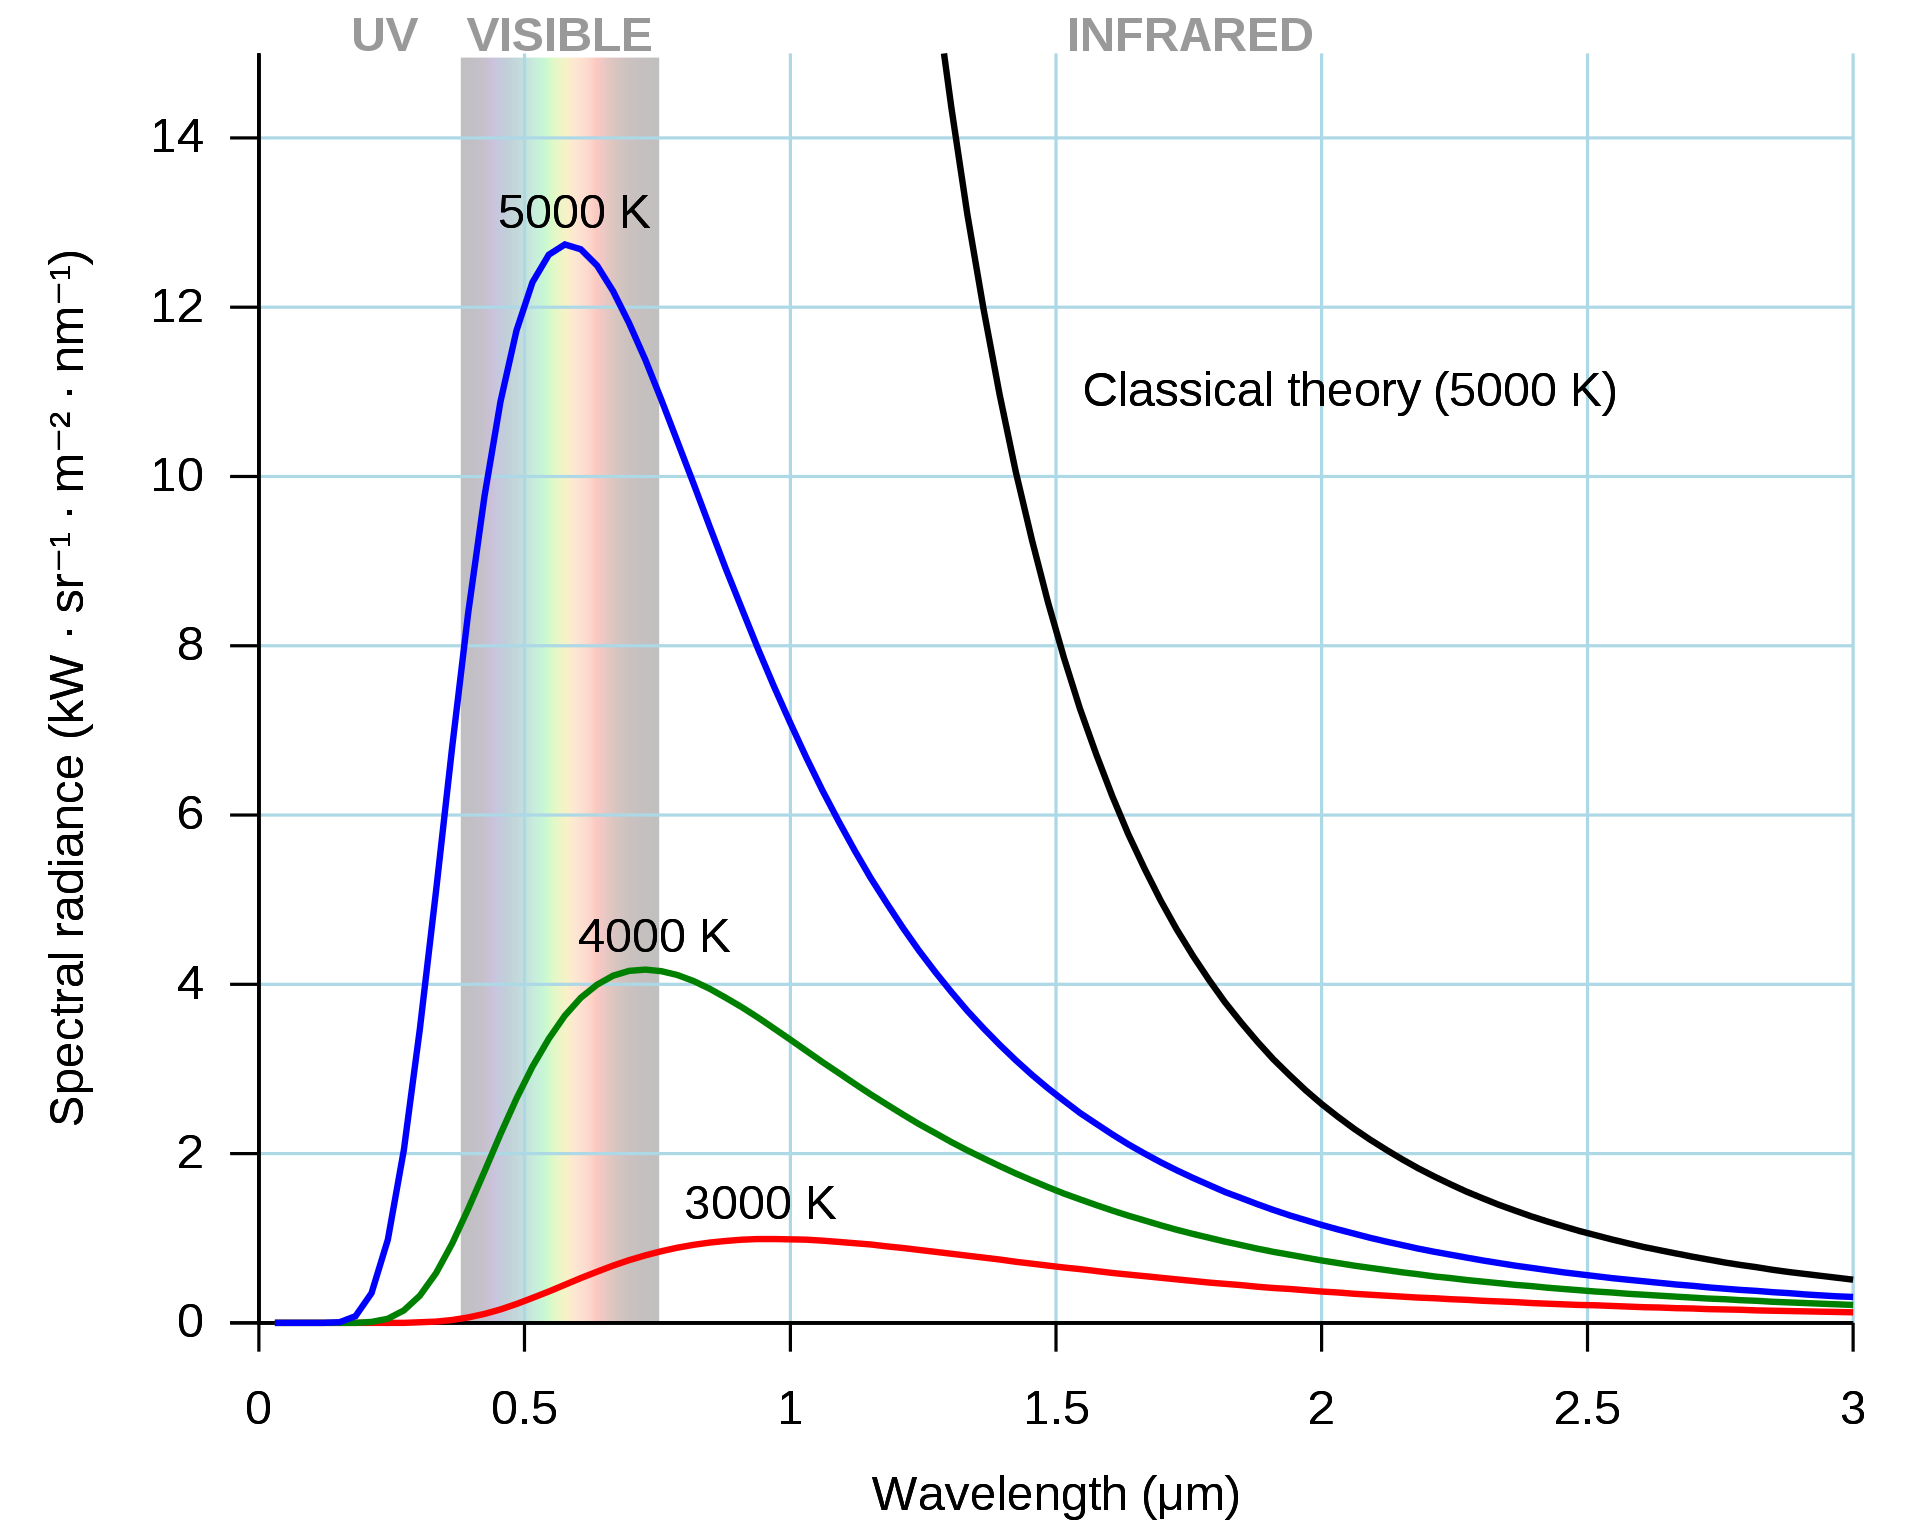
\includegraphics[width=\linewidth]{Figures/black_body_spectrum.png}
    \caption{Φάσμα εκπομπής μελανών σωμάτων διαφόρων θερμοκρασιών. Στα μικρά μήκη κύματος φαίνεται η υπεριώδης καταστροφή (UV catastrophe) όπως προκύπτει με την κλασική θεωρία των Rayleigh-Jeans.}
    \label{fig:black_body_spectrum}
\end{figure}

Παρατηρώντας τα φάσματα του σχήματος \ref{fig:black_body_spectrum} βλέπουμε ότι:

\begin{enumerate}
    \item Η ακτινοβολία μέλανου σώματος είναι συνεχής
    \item $T_1 < T_2 < T_3 \Rightarrow \lambda_1 > \lambda_2 > \lambda_3$
    Αυτό σημαίνει ότι υπάρχει ένα μήκος κύματος όπου η ακτινοβολία γίνεται μέγιστη και μάλιστα,  μέλανα σώματα υψηλότερης θερμοκρασίας εκπέμπουν ακτινοβολία μικρότερου μήκου κύματος.
    \item {\color{red} Οι καμπύλες δεν τέμνονται ποτέ!} Ένα μέλαν σώμα υψηλότερης θερμοκρασίας θα εκπέμπει \underline{πάντα} περισσότερη ακτινοβολία συγκριτικά με ένα μέλαν σώμα χαμηλότερης θερμοκρασίας. Το μόνο που συμβαίνει είναι ότι το μέγιστο της εκπομπής μετακινείται σε υψηλότερα μήκη κύματος.
\end{enumerate}

\subsection{Νόμος του Planck}
Ποιά είναι όμως η συνάρτηση που δίνει τις καμπύλες (φάσμα) ενός μέλανος σώματος;
Η ένταση του φωτός που παράγει ένα μέλαν σώμα θερμοκρασίας Τ σε μήκος κύματος $\lambda$, δίνεται από τη σχέση του Planck:

\begin{equation}
    \label{eq:planck_function_lambda}
    B_{\lambda}(T) = \frac{2hc^2}{\lambda^5} \frac{1}{\exp(hc/\lambda kT) - 1}
\end{equation}

Η παραπάνω σχέση είναι γνωστή ως \textit{νόμος του Planck}. Μπορούμε να εκφράσουμε το νόμο του Planck με όρους συχνότητας, αλλά δεν αρκεί η αντικατάσταση του μήκους κύματος με τη συχνότητα σύμφωνα με τη θεμελιώδη σχέση $\nu \lambda = c$. Αυτό που πρέπει να θυμόμαστε είναι ότι {\color{blue} ο νόμος του Planck εκφράζει ενέργεια ανα μονάδα χρόνου, ανα επιφάνεια, ανα μήκος κύματος (ή συχνότητα), και ανα στερεά γωνία}. Οπότε πρέπει να ισχύει:

\begin{eqnarray*}
    B_{\lambda} (T) &=& \frac{dE}{dt \cdot dA \cdot d \lambda \cdot d \Omega} \\ 
    B_{\nu} (T) &=& \frac{dE}{dt \cdot dA \cdot d \nu \cdot d \Omega} \\\\
    &\text{ή}& \\\\
    |B_{\lambda} (T) d \lambda | &=& |B_{\nu} (T) d \nu |
\end{eqnarray*}
Άρα αν ολοκληρώσουμε σε όλα τα μήκη κύματος/συχνότητες παίρνουμε την ολική ενέργεια που εκπέμφθηκε. Αλλά: $$\nu \lambda = c \Rightarrow \nu = \frac{c}{\lambda} \Rightarrow |d\nu | = | d \left( c / \lambda \right) | \Rightarrow | d\nu | = \left | \frac{c}{\lambda^2}d\lambda \right |$$

Τελικά έχουμε:

\begin{eqnarray}
\label{eq:planck_function_frequency}
    B_{\nu}(T) &=& \frac{B_{\lambda}(T) d \lambda}{d\nu} \Rightarrow B_{\nu}(T) = \frac{B_{\lambda}(T) \cancel{d\lambda}}{\displaystyle  \frac{c}{\lambda^2} \cancel{d \lambda}} =  \frac{\lambda^2}{c} \frac{2hc^2}{\lambda^5} \frac{1}{\exp(hc / \lambda kT) - 1} \Rightarrow \nonumber \\ \nonumber \\
    &\Rightarrow & B_{\nu}(T) =  \frac{2hc}{\lambda^3} \frac{1}{\exp(hc / \lambda kT) - 1} =  \frac{2hc}{c^3 / \nu^3} \frac{1}{\exp(h \nu / kT) - 1} \Rightarrow \nonumber \\ \nonumber \\
    &\Rightarrow & \boxed{B_{\nu}(T) =  \frac{2h \nu^3}{c^2} \frac{1}{\exp(h \nu / kT) - 1}}
\end{eqnarray}


\subsection{Νόμος του Wien}
Αν διαφορίσουμε τη συνάρτηση του Planck (σχέση \eqref{eq:planck_function_lambda}) ως προς μήκος κύματος και τη θέσουμε ίση με μηδέν, παρατηρούμε ότι φτάνει ένα μέγιστο σε μήκος κύματος:
$$\frac{d B_{\lambda}(T)}{d \lambda} = 0 \Rightarrow \lambda_{\text{max}} = 0.2 \frac{hc}{kT} = \frac{0.29}{T} \ \text{cm}$$

\begin{equation}
    \boxed{\lambda_{\text{max}} \cdot T = 0.003 \ \text{mK}}
\end{equation}

Άρα το μήκος κύματος στο οποίο η εκπομπή ακτινοβολίας είναι μέγιστη εξαρτάται \underline{μόνο} από τη θερμοκρασία $\longrightarrow$ άρα δεν έχουν όλα τα αστέρια την ίδια επιφανειακή θερμοκρασία.

\subsection{Νομος των Stefan-Boltzmann}
Ολοκληρώνοντας αυτή τη φορά τον νόμο του Planck για όλες τις συχνότητες, προκύπτει ότι:

\begin{equation}
    \label{eq:stefan_boltzmann}
    L = A \sigma T^4 \Rightarrow \boxed{L = 4 \pi R^2 \sigma T_{\text{eff}}^4}
\end{equation}
όπου $A$ είναι η επιφάνεια μέλανος σώματος, και για αστέρα ακτίνας $R$ ισχύει $A=4\pi R^2$. Ο παράγοντας $T_{\text{eff}}^4$ ονομάζεται \textit{ενεργός θερμοκρασία} του αστέρα και ορίζεται ως η θερμοκρασία που θα έπρεπε να έχει ένα μέλαν σώμα ώστε να παράγει την ίδια ροή ενέργειας που παράγει η επιφάνεια του αστέρα. Με άλλα λόγια η ενεργός θερμοκρασία προσεγγίζει ικανοποιητικά την θερμοκρασία της επιφάνειας του αστέρα.

Γίνεται αντιληπτό ότι αν γνωρίζω την απόσταση ενός αστέρα (π.χ. μέσω της παράλλαξης), την φωτεινότητά του (με φωτομετρικές παρατηρήσεις) μπορώ να υπολογίσω τη λαμπρότητά του. Γνωρίζοντας την λαμπρότητα του αστέρα και μετρώντας την $T_{\text{eff}}^4$ (νόμος Wien) μπορώ να έχω μία εκτίμηση για την ακτίνα του αστέρα μέσω της σχέσης \eqref{eq:stefan_boltzmann}.

Τέλος, η εκπεμπόμενη ροή ακτινοβολίας από την επιφάνεια του αστέρα θα είναι:

\begin{eqnarray}
    F_{\text{surface}} = \frac{L}{4 \pi R^2} = \frac{\cancel{4 \pi R^2} \sigma T_{\text{eff}}^4}{\cancel{4 \pi R^2}} \Rightarrow F_{\text{surface}} = \sigma T_{\text{eff}}^4
\end{eqnarray}

